\clearpage
\chapter{Experimentations, Réalisations}
\label{sec:exp}

\section{Représentation Graphe/Squelette porteuse de sens}
\label{dfs}
\subsection{Introduction}
Le format de structure de données de la majorité des articulations disponibles via les approches de squelettisation en un tenseur ignore les relations de dépendance physique entre les articulations et ajoute de fausses connexions entre les articulations du corps qui ne sont pas liées physiquement.

\begin{figure}[H]
    \centering
    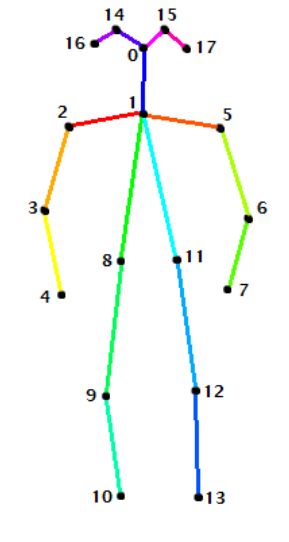
\includegraphics[width=0.3\linewidth]{Images/openpose.png}
    \caption{Structure de données de la représentation squelette obtenue à l'aide de la bibliothèque OpenPose \cite{cao2017realtime}}
    \label{fig:openPoseSkel}
\end{figure}

La figure \ref{fig:openPoseSkel}, nous permet de constater que conserver le squelette obtenu par les algorithmes de détection de pose classiques, sans avoir recours à une transformation pourrait réduire la qualité de nos résultats: certains couples d'articulations, bien que se suivant de manière incrémentale dans la structure de données utilisée, n'ont en réalité aucune raison valable de l'être: par exemple, l'extrémité gauche du bras et l'épaule droite (\textit{nodes 4 et 5}) ou encore l'extrémité droite du bras et la hanche gauche (\textit{nodes 7 et 8}).

Une grande majorité des travaux actuels semblent négliger l'importance de cette représentation spatiale et ne se focalisent que sur le coté temporel: la dynamique des articulations, sans remettre en question la structure de données spatio-temporelle en entrée.

\subsection{Méthodologie}

En reprenant les travaux de \cite{liu2016spatio} et \cite{2018arXiv180110304Y}, j'ai souhaité m'intéresser à cette question de représentation: en réalisant un Depth-First Search (DFS) sur un hub du graphe représentant le squelette. De cette manière, il est possible d'obtenir une structure de type arbre/graphe n'exploitant que des liens de voisinage entre joints existants.



\algnewcommand\algorithmicforeach{\textbf{for each}}
\algdef{S}[FOR]{ForEach}[1]{\algorithmicforeach\ #1\ \algorithmicdo}

\begin{algorithm}
 \caption{Explorer}\label{algorithm1}
 \KwIn{graphe G, sommet s}
  marquer le sommet s\;
  afficher(s)\;
 \ForEach {sommet $t$ fils de $s$}{
  \eIf{$t$ n'est pas marqué}{
    Explorer(G,t)\;
  }
 }
\end{algorithm}


\begin{algorithm}
 \caption{Depth-First Search (DFS)}\label{algorithm1}
 \KwIn{graphe G}
 %\KwOut{how to write algorithm with \LaTeX2e }
 %initialization\;
 \ForEach {sommet $s \in \mathcal G $}{
  \eIf{s n'est pas marqué}{
    explorer(G,s)\;
  }
 }
\end{algorithm}

L'exploration d'un DFS depuis un sommet $s$ fonctionne comme suit. L'algorithme poursuit  un chemin dans le graphe jusqu'à une feuille ou jusqu'à atteindre un sommet déjà visité. L'algorithme revient alors sur le dernier sommet où il était possible de suivre un autre chemin puis continue d'explorer. L'exploration s'arrête quand tous les sommets depuis $s$ ont été visités.

Ainsi, en reprenant la structure de données format tenseur d'un jeu de données, il est possible de réaliser un DFS afin d'obtenir une représentation respectant les relations de dépendance physique du squelette (\ref{fig:DFS}).

\begin{figure}[H]
    \centering
    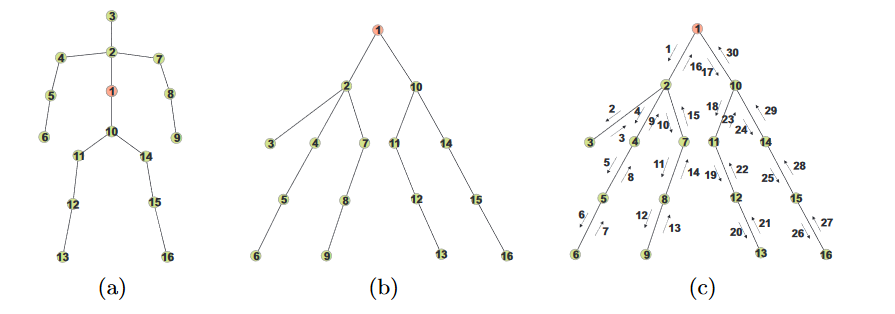
\includegraphics[width=1\linewidth]{Images/DFS.png}
    \caption{(a) Articulations du squelette d'un corps humain avec la structure de données initiale. L'ordre de visite des noeuds est incrémentale:1-2-3-...-16. (b) Le squelette est transformé en une structure arborescente. (c)  L'arbre peut être dépilé en une chaîne dont l'ordre de visite des noeuds conserve la relation physique des articulations: 1-2-3-2-4-5-6-5-4-2-7-8-9-8-7-2-1-10-11-12-13-12-11-10-14-15-16-15-14-10-1, Figure équivalente à la figure 2 dans  \cite{liu2016spatio}.}
    \label{fig:DFS}
\end{figure}


L'idée derrière cette normalisation précédant l'application de convolutions est que la fenêtre de la convolution ne se focalise que  sur des features dont les keypoints sont liés physiquement dans la réalité tout en évitant le plus de redondance, inévitable lorsque l'on souhaite conserver la structure spatiale. Comme présenté sur la figure \ref{fig:explanationCNN}, les keypoints étant organisés pour respecter la structure spatio-temporelle de l'action, dans le cadre d'une convolution 1D, la fenêtre se focalisera par exemple sur trois keypoints tels que le genou, le pied et la hanche et de leur position pour tout instant de la séquence. Dans le cadre d'une convolution 2D, nous ajoutons une limite à la séquentialité pour la fenêtre et celle-ci se focalisera sur un nombre figé de pas de temps et non la totalité de la séquence.



\begin{figure}[H]
    \centering
    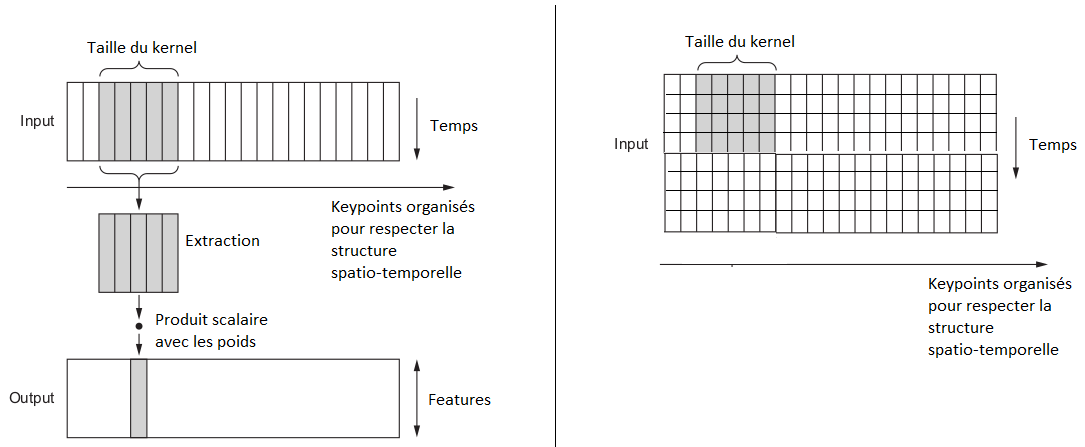
\includegraphics[width=0.95\linewidth]{Images/explanation_cnn_dfs.png}
    \caption{Explication de la formalisation des données en un tenseur sous pour une convolution 1D et convolution 2D et visualisation de l'application d'un CNN pour de telles données.}
    \label{fig:explanationCNN}
\end{figure}

Souhaitant m'intéresser à la plus-value apportée par cette représentation proposée par \cite{liu2016spatio} et \cite{2018arXiv180110304Y} pour la classification d'actions squelettiques, j'ai souhaité me comparer à un modèle de classification existant pour les mêmes conditions expérimentales dans le cadre de convolutions 1D et convolutions 2D. Je me suis donc basé sur l'approche expérimentale de Double-feature Double-motion Network \cite{2019arXiv190709658Y} ainsi que sur leur architecture présentée en \ref{fig:DDnet} pour les CNN 1D et avec un simple Lenet-5 \cite{lecun1998gradient} pour les convolutions 2D dont l'architecture est présentée en \ref{fig:Lenet}.


\begin{figure}[H]
    \centering
    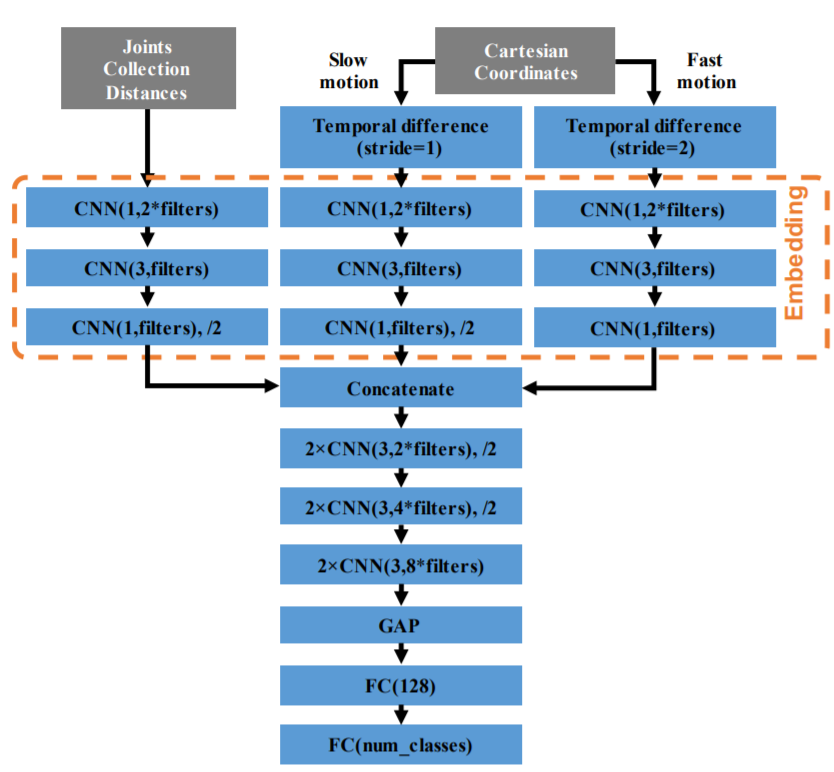
\includegraphics[width=0.55\linewidth]{Images/ddnet.png}
    \caption{L'architecture du réseau DD-Net. \textit{2×CNN(3,
2*filters),/2} désigne deux couches 1D ConvNet (taille du noyau
= 3, channels = 2*filtres) et un Maxpooling (strides = 2).GAP
désigne le Global Average Pooling. FC signifie "Fully Connected". La taille du modèle est ajustable en fonction de la variable \textit{filters}.}
    \label{fig:DDnet}
\end{figure}

\begin{figure}[H]
    \centering
    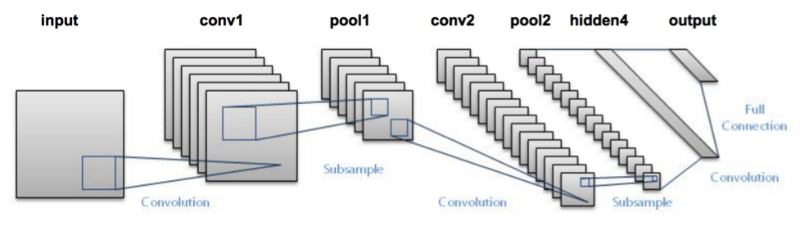
\includegraphics[width=0.85\linewidth]{Images/lenet_architecture.png}
    \caption{L'architecture du réseau LeNet, possédant les unités de base d'un réseau convolutif: convolutions, pooling, fully connected layer et softmax.}
    \label{fig:Lenet}
\end{figure}

\subsection{Tests et évaluations}
\label{JHMDBSHREC}
\subsubsection{Evaluation datasets et protocole d'évaluation}

Nous avons expérimenté les capacités de cette représentation sur deux jeux de données de reconnaissances d'action squelettiques: SHREC (actions de la main en 3D) proposé par \cite{de2017shrec} et JHMDB (action du corps en 2D)  proposé par \cite{jhuang2013towards}.\\

Similairement à \cite{2019arXiv190709658Y}, SHREC est évalué pour deux cas : pour 14 et 28 gestes. L'ensemble de données JHMDB est évalué en utilisant des squelettes annotés manuellement, et l'évaluation se fait par cross-validation sur un split 3.

\subsubsection{Détails d'implémentation}

\begin{itemize}
    \item \textbf{Modèle CNN 1D}: Les conditions expérimentales ne diffèrent pas de celles de \cite{2019arXiv190709658Y}.
    \item \textbf{Modèle CNN 2D}: Nous disposons pour chaque instance d'un tenseur de dimension 3: (32, 22, 3) et de dimension (32, 43, 3) pour la version DFS. Ces valeurs correspondent respectivement au nombre de frames, au nombre de keypoints et à leur position dans l'espace 3d pour une action donnée. L'image d'entrée est arrangée selon l'approche présentée dans la figure \ref{fig:skeltoim} du chapitre \ref{partieconvolutive}. \newline Contrairement à l'architecture Lenet \cite{lecun1998gradient} originale, nous ajoutons pour chaque layer une couche de dropout de valeur \textit{0.5}. Après l'extraction de features des couches convolutives, une couche de batchnormalisation est ajoutée pour chaque layer dense de l'architecture préalablement au dropout.\newline L’entraînement est réalisé avec l'optimiseur Adam \cite{kingma2014adam} suivant les recommandations du papier initial et avec un learning rate de 0.01. Nous réduisons automatiquement le learning rate de moitié une fois coincé dans un plateau après 5 epochs n'améliorant pas la loss.
\end{itemize}



\subsubsection{Résultats}

\begin{itemize}
    \item \textbf{Modèle CNN 1D}:
    \begin{table}[H]
\centering
\scalebox{0.75}{
\begin{tabular}{l|l|l|l} 
\hline
\textbf{Méthode}               & \textbf{Paramètres} & \textbf{14 classes} & \textbf{28 classes}  \\ 
\hline
DD-NET (64 filtres)     & 1.82M               & 94.6\%              & 91.9\%               \\
DD-NET (32 filtres)     & 0.50M               & 93.5\%              & 90.4\%               \\
DD-NET (16 filtres)     & 0.15M               & 91.8\%              & 90.0\%               \\ 
\hline
DFS-DD-NET (64 filtres) & 1.84M               & \textbf{95.9}\%              &  \textbf{92.4}\%                   \\
DFS-DD-NET (32 filtres) & 0.51M               & 94.7\%              &  92.0\%                   \\
DFS-DD-NET (16 filtres) & 0.16M               & 93.1\%              &  90.5\%                   
\end{tabular}
}
\caption{Résulats obtenus grâce à la normalisation DFS sur SHREC \cite{de2017shrec} (Squelettes de main 3D) en conservant l'architecture \cite{2019arXiv190709658Y}}
\end{table}

\begin{table}[H]
\centering
\scalebox{0.75}{
\begin{tabular}{l|l|l}
\hline
\textbf{Méthode}       & \textbf{Paramètres} & \textbf{Resultats}  \\ 
\hline
Chained Net \cite{2017arXiv170400616Z}             & 17.5M           & 56.8\%              \\
EHPI \cite{ludl2019simple}                   & 1.22M           & 65.5\%              \\
POTION    \cite{choutas2018potion}              & 4.87M            & 67.9\%              \\
DD-Net (filters 64)     & 1.82M           & \textbf{77.2}\%              \\
DD-Net (filters 32)     & 0.5M            & 73.7\%              \\
DD-Net (filters 16)     & 0.15M           & 65.7\%              \\ 
\hline
DFS-DD-NET (filters 64) & 1.81M               & 76.7\%                  \\
DFS-DD-NET (filters 32) & 0.5M               & \textbf{77.2}\%                  \\
DFS-DD-NET (filters 16) & 0.15M           & 66.4\%                 
\end{tabular}}
\caption{Résulats obtenus grâce à la normalisation DFS en conservant l'architecture \cite{2019arXiv190709658Y} sur JHMDB \cite{jhuang2013towards} (Squelettes corps humain 2D)}
\end{table}
    
    \item \textbf{Modèle CNN 2D}:
    \begin{table}[H]
\centering
\scalebox{0.75}{
\begin{tabular}{l|l|l|l|l} 
\hline
\textbf{Méthode} & \textbf{Kernel Size} & \textbf{Params} & \textbf{accuracy 14} & \textbf{accuracy 28}  \\ 
\hline
Lenet-5          & 3x3                  & 0.10M           & 90.9\%               & 83.8\%                    \\
Lenet-5          & 5x5                  & 0.10M           & 91.9\%               & 85.5\%                    \\
Lenet-5          & 7x7                  & 0.10M           & 92.3\%                   & 84.5\%                    \\ 
Lenet-5          & 9x9                  & 0.10M           & 90.9\%                   & 87.6\%                    \\ 
\hline
DFS-Lenet-5      & 3x3                  & 0.18M           & 90.9\%               & \textbf{89.1}\%                    \\
DFS-Lenet-5      & 5x5                  & 0.18M           & 92.9\%               & 88.1\%                    \\
DFS-Lenet-5      & 7x7                  & 0.18M           & \textbf{93.4}\%               & 88.6\%                  \\
DFS-Lenet-5      & 9x9                  & 0.18M           & 91.5\%               & 87.6\%                   
\end{tabular}}
\caption{Résulats obtenus grâce à la normalisation DFS sur SHREC \cite{de2017shrec} (Squelettes de main 3D) pour un réseau convolutif 2D: Lenet.}
\end{table}


\begin{table}[H]
\centering
\scalebox{0.75}{
\begin{tabular}{l|l|l|l} 
\hline
\textbf{Méthode} & \textbf{Taille de kerne}l & \textbf{Paramètres} & \textbf{accuracy}  \\ 
\hline
Lenet-5          & 3x3                       & 0.07M               & 65.1\%             \\
Lenet-5          & 5x5                       & -                   & 67.7\%             \\
Lenet-5          & 7x7                       & -                   & 69.7\%             \\
Lenet-5          & 9x9                       & -                   & 69.4\%             \\ 
\hline
DFS-Lenet-5      & 3x3                       & 0.13M               & 63.5\%             \\
DFS-Lenet-5      & 5x5                       & -                   & 65.2\%             \\
DFS-Lenet-5      & 7x7                       & -                   & \textbf{71.9\%}    \\
DFS-Lenet-5      & 9x9                       & -                   & 68.1\%            
\end{tabular}}
\caption{Résulats obtenus grâce à la normalisation DFS sur JHMDB \cite{jhuang2013towards} (Squelettes corps humain 2D) pour un réseau convolutif 2D: Lenet.}
\end{table}
\end{itemize}

\subsubsection{Discussion}

Nous remarquons ici, une amélioration de l'accuracy pour deux jeux de données traitant des problèmes similaires: la reconnaissance d'action squelettiques pour des niveaux différents (la main et le corps), pour des dimensions différentes (2d et 3d) et pour des dimensions de convolutions variantes.

La normalisation semble fonctionner plus significativement sur le jeu de données SHREC comparé à JHMDB. Une explication plausible serait que le niveau d'abstraction et de précision n'est pas le même entre ces jeux de données. Le nombre de keypoints dans SHREC est supérieur à JHMDB et par conséquent l'organisation de ceux-ci pourrait apporter plus d'information. 

En choisissant volontairement un modèle complexe pour la convolution 1d et un modèle trivial pour la convolution 2d. Nous émettons l'hypothèse que cette transformation peut-être bénéfique peu importe le niveau de complexité du modèle. Cependant, celle-ci modifie significativement la taille de l'entrée du réseau et par conséquent la taille en paramètres des approches augmentera. Cette augmentation n'est que peu visible sur DD-Net car il n'y a pas de layer dense. Pour Lenet-5 la taille du modèle augmente du simple au double, et ce à cause de la partie fully connected de l'architecture. Il conviendra donc d'éviter le plus possible l'utilisation de layer dense pour cette approche ou de travailler sur des réseaux de taille réduite.

Finalement, cette normalisation nécessite une connaissance à priori de l'organisation de la structure des données en entrée (coude: keypoint 1, tête: keypoint 2, ...). Dans le cadre de la thèse, cela ne pose pas de contraintes spécifiques. Cependant, il sera par exemple impossible de réaliser ce travail sur des jeux de données dont la structure des données n'est pas précisée.

\section{Autoencodeur semi-supervisé pour l'action recognition}
\label{refAEmod}

\subsection{Introduction}
Les auto encodeurs étant une composition de transformation non linéaires en esperant trouver une représentation dans l'espace adaptée au format des données et conservant un maximum de sémantique de celui-ci.

Je me suis intéréssé à cette question de représentation pour plusieurs raisons:
\begin{itemize}
    \item Tout est une question d'embedding et de normalisation en machine learning. Le role premier des couches cachées est de transformer cet embedding en espérant qu'il soit porteur d'information. Le jour où l'on trouve un moyen de normaliser et de représenter les données de manière plus adéquate, n'importe quel classifieur pourra obtenir de bons résultats pour peu que les données en entrée soient porteuses d'information. Le jour où l'on arrivera à obtenir une représentation utilisable plus rapidement au lieu de stacker des layers au sein d'un réseau de neurones, d'autres problématiques d'apprentissage apparaîtront mais le gain serait intéressant: (Selon le théorème d'approximation universelle, n'importe quel Shallow Network peut supposément approximer une fonction donnée \cite{universalapproxtheorm,scarselli1998universal}). 
    
    \item En s’intéressant à la question de la représentation des données, on évite un apprentissage de cette représentation à "l'aveugle": en optimisant un réseau précis sur un jeu de données précis et en testant un maximum d’hyper-paramètres on est assurés de faire un bon résultat. Plus la représentation des données est fiable, plus l'architecture utilisée pour la classification peut-être triviale.
    On peut donc potentiellement réduire la taille de notre réseau et donc par définition réduire le temps d'inférence de celui-ci, ce qui peut être intéressant dans le cadre d'un sujet en temps réel.
    
    \item Peu de travaux de recherche en reconnaissance d'actions se focalisent sur la représentation des données, la majorité des travaux actuels translatent la connaissance de domaines connexes tels que la computer vision ou le text-mining et s'inspirent des méthodes de l'état de l'art dans ces domaines. Il n'existe à ce jour à ma connaissance aucune publication sur l'utilisation des auto-encodeurs pour la reconnaissance d'actions squelettiques.
\end{itemize}

L'idée étant d’entraîner un auto-encodeur avec une fonction de coût modifiée en rajoutant une contrainte sur la séparation linéaire des classes dans l'espace latent (LDA / QDA / FDA). Il a été montré que la représentation optimale interne d'un MLP s'obtient en faisant une analogie avec une analyse discriminante non linéaire \cite{webb1990optimised}. Parallèlement, \cite{2020arXiv200312843B} montrent que l'ajout d'une fonction de coût non-supervisée lors d'un problème de classification avec peu de données permet une meilleure généralisation des réseaux.


Les approches factorielles citées plus haut s'apparentent à la projection de données dans l'espace comme celle d'une ACP mais tandis que l'ACP maximise la variance du jeu de données, celles-ci se focalisent sur la maximisation de la séparabilité des classes dans l'espace, ce qui en fait des méthodes supervisées. On obtiendrait donc un Auto-encodeur "semi-supervisé" dans le sens où celui-ci se focalise sur deux informations complètement différentes dans les données, l'une de manière non-supervisée, l'autre de manière supervisée:
\begin{itemize}
    \item La structure inhérente des données capturée de manière non supervisée grâce à la reconstruction de l'Auto-encodeur et sa capacité d'abstraction. On conserverait alors une partie de l'information importante et discriminante du jeu de données. (feature extraction)
    \item La séparabilité des classes dans l'espace grâce à l'analyse discriminante (non) linéaire. Ce qui permettrait de réduire le nombre de layers.
\end{itemize}{}


Nous pouvons imaginer deux utilisations à cette approche:
\begin{itemize}
    \item Récupérer cet espace latent combinant les informations "data driven" grâce à l'apprentissage non-supervisé de l'auto encodeur classique et la première ébauche de séparabilité linéaire grâce à la seconde partie de la fonction de coût. Envoyer l'espace latent à un réseau de neurones très peu profond pour la classification. Finetuner le réseau de bout en bout et voir ce que cela apporte quand à la capacité de discrimination de l'approche. 
    \item Générer des données en réalisant une génération d'instances au niveau de l'espace latent grâce à des approches type SMOTE \cite{chawla2002smote} ou ADASYN \cite{he2008adasyn}  et utiliser la partie décodeur pour  faire de la data génération.
\end{itemize}

\subsection{Formalisation}
La pipeline complète de notre approche est présentée en figure \ref{fig:AEmodif}.
Nous définissons le problème comme ceci: \newline
$$\min _{\theta_{1}, \theta_{2}},\left\|\mathbf{X}-g_{\theta_{2}}\left(f_{\theta 1}(\mathbf{X})\right)\right\|^{2}$$

Fonction de reconstruction habituelle d'un auto-encodeur avec $\theta_{1}, \theta_{2}$ les paramètres des blocs encodeur et décodeur de l’AE. 

$$\min _{\theta_{1}, \theta_{2}, \mathbf{S}}\left\|\mathbf{X}-g_{\theta_{2}}\left(f_{\theta_{1}}(\mathbf{X})\right)\right\|^{2}+\lambda\left\|f_{\theta_{1}}(\mathbf{X})-\mathbf{S}_{f_{\theta 1}}(\mathbf{X})\right\|^{2}$$

Ajout d'une variation dans la fonction de coût: avec S la matrice de projection des individus dans l'espace latent obtenue avec une analyse discriminante linéaire (LDA) et $\lambda$ un régularisateur.

Une fois, l’entraînement de l’auto-encodeur réalisé, récupération des poids de la partie encodeur: $f_{\theta 1}$, ajout d'une fonction classifieur softmax:\\ 


\begin{figure}[H]
    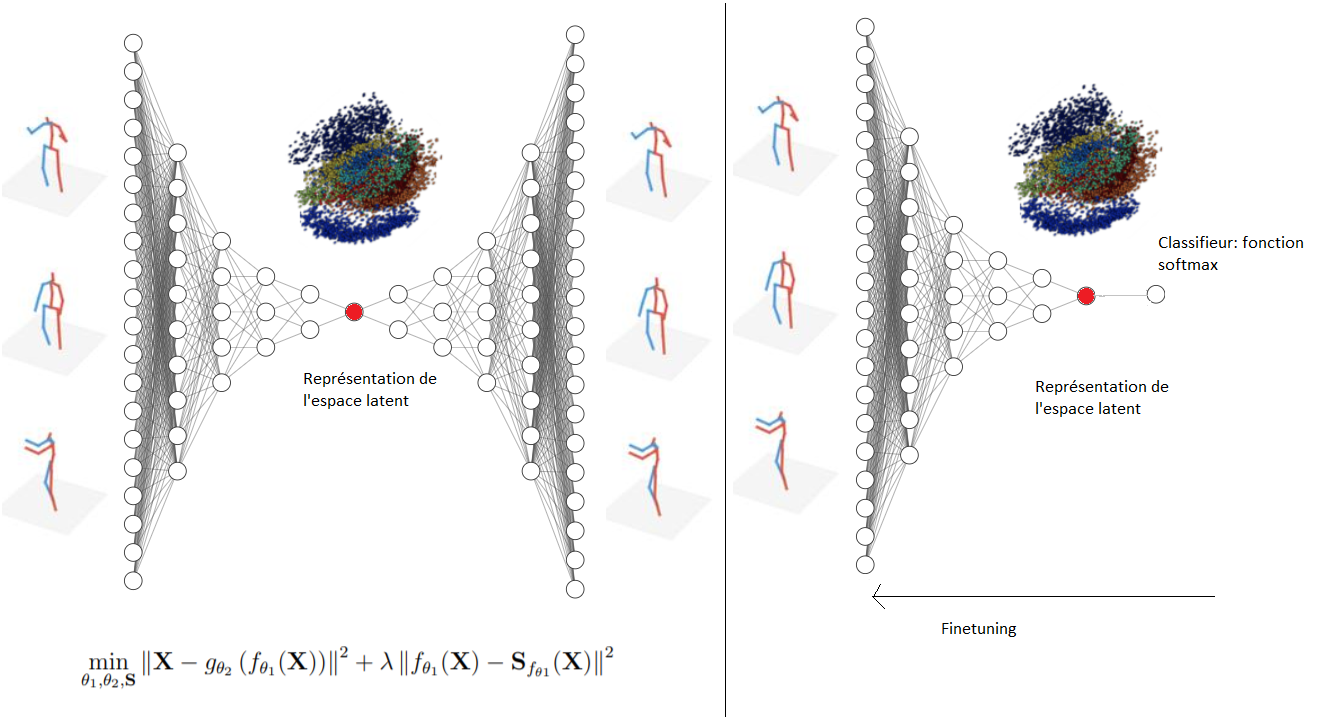
\includegraphics[width=1.1\linewidth]{Images/AE_supervis.png}
    \caption{Pipeline de l'approche: (1) nous entraînons un auto-encodeur pour reconstruire une séquence représentant une action en y ajoutant une contrainte spécifique à la séparabilité des classes dans l'espace latent. (2) extraction des poids de la partie encodeur jusqu'au bottleneck représenté en rouge et ajout d'une softmax, transformant alors la partie encodeur en un réseau pré-entraîné sur les données pour la classification des actions.}
    \label{fig:AEmodif}
\end{figure}

Nous souhaitons dans un premier temps évaluer l'apport de cette représentation pour la classification.

\subsection{Tests et évaluation}

\subsubsection{Evaluation datasets}
Par soucis d'économie de temps, j'ai réalisé l'évaluation de cette approche sur les mêmes jeux de données que ceux présentés en \ref{JHMDBSHREC}, à savoir SHREC \cite{de2017shrec} et JHMDB \cite{jhuang2013towards}.\\

\subsubsection{Détails d'implémentation}

Afin d'évaluer la qualité de représentation, nous avons choisi de prendre une architecture d'autoencodeur la plus facile possible: semblable à celle d'un perceptron multicouches. Naturellement, il est possible de réaliser le même travail sur des auto-encodeurs convolutifs ou séquentiels afin de capturer la séquentialité de l'action ou de minimiser la taille du réseau et ainsi potentiellement améliorer l'accuracy et le temps d'inférence.\\

L'architecture est composée d'une partie encodeur et d'une partie décodeur.
La partie encodeur est définie telle quelle:
\begin{itemize}
    \item Un couche d'entrée de dimension 2112 représentant les valeurs d'une action complète pour 32 pas de temps, 22 keypoints et  3 dimensions.
    \item 5 layers dense d'extractions de features dont la dimension diminue d'une puissance de deux pour chaque layer (512, 256, 128, 64, 32).
    \item Un bottleneck de dimension du nombre de classe du jeu de données moins un: le nombre maximum d'axes obtenus par les analyses factorielles correspond au nombre de classe moins un. Pour SHREC 14 celui-ci aura 13 valeurs pour SHREC 28 27 valeurs et pour JHMDB 20 valeurs.
\end{itemize}

La partie décodeur est symétrique à la partie encodeur à l'exception du bottleneck qui est unique.\\
Pour chaque layers, nous ajoutons une couche de dropout de valeur \textit{0.1} et de la batchnormalisation préalablement au dropout.
L’entraînement est réalisé avec l'optimiseur Adam \cite{kingma2014adam} suivant les recommandations du papier initial pour la première et la seconde étape.\\

L'optimisation du paramètre $\lambda$ est actuellement sujette à discussions, nous avons pour l'instant fait varier les valeurs de lambda de manière empirique afin de suivre l'impact que la normalisation LDA avait sur le résultat final. 

\subsubsection{Résultats}

\begin{table}[H]
\centering
\scalebox{0.75}{
\begin{tabular}{l|l|l|l|l}
\hline
\textbf{Méthode}                                 & \textbf{Nb Params} & \textbf{SHREC 14} & \textbf{SHREC 28} & \textbf{FPS (RTX 2080 ti)}  \\ 
\hline
LDA sur l'input                   &          - &         33.0\% &          27.6\%&      \\
LDA sur le bottleneck AE classique (\lambda = 0)              &          - &         37.9\% &          42.8\%&      \\
LDA sur le bottleneck AE modifié (\lambda = 5)              &          - &         43.5\% &          35.6\%&      \\
\hline
MLP Sans initialisation                      &          1.2M &         91.2\% &          85.2\%&     20 000 \\
MLP Avec initialisation AE classique (\lambda = 0)        &          1.2M &          91.5\%&          85.9\%&      -\\
MLP Avec initialisation AE Modifié (\lambda =1) &          1.2M &          91.9\%&          87.6\%&      -\\
MLP Avec initialisation AE Modifié (\lambda = 2.5) &           1.2M&          92.4\%&          86.9\%&     -\\
MLP Avec initialisation AE Modifié (\lambda = 5)          &          1.2M &          \textbf{92.5\%}&         \textbf{87.1}\% &      -\\
MLP Avec initialisation AE Modifié (\lambda = 7.5) &          1.2M &         91.9\% &          86.4\%&      -\\
MLP Avec initialisation AE Modifié (\lambda = 10) &          1.2M &          90.9\%&          85.2\%&      -


\end{tabular}}
\label{trivial}
\caption{Résulats obtenus grâce à l'initialisation des poids avec un AE modifié sur SHREC \cite{de2017shrec}}
\end{table}




\begin{table}[H]
\scalebox{0.7}{
\centering
\begin{tabular}{l|l|l|l} 
\hline
\textbf{Methode}                  & \textbf{Nb Params} & \textbf{\textcolor[rgb]{0.129,0.145,0.161}{Average accuracy of 3 splits ~})\textcolor[rgb]{0.129,0.145,0.161}{}~} & \textbf{Classifications par secondes}  \\
\hline
Chained Net (ICCV17)              & 17.50 M            & 56.8\%                                                                                                                                        & 33 (1080 Ti)                           \\
EHPI~ (ITSC19)                    & 1.22 M             & 65.5\%                                                                                                                                        & 29 (1080 Ti)                           \\
PoTion (CVPR18)                   & 4.87 M             & 67.9\%                                                                                                                                        & 100 (1080 Ti)                          \\
DD-Net                            & 1.82M              & 77.2\%                                                                                                                                        & 2,200 (1080 Ti)                        \\ 
\hline
Sans initialisation (\lambda =0)~ & 0.67M                  &   65.2\%                                                                                                                                            & -                                      \\

Avec initialisation AE classique (\lambda =0)~ & 0.67M                  &   66.4\%                                                                                                                                            & -                                      \\
Avec initialisation AE modifié (\lambda =1)    & -                  &          66.2\%                                                                                                                                     & -                                      \\
Avec initialisation AE modifié (\lambda =2.5)   & -                  &          68.3\%                                                                                                                                     & -                                      \\
Avec initialisation AE modifié (\lambda =5)   & -                  &        67.9\%                                                                                                                                       & -                                      \\
Avec initialisation AE modifié (\lambda =7.5)   & -                  &          66.5\%                                                                                                                                     & -                                      \\
\hline
\end{tabular}}
\caption{Résulats obtenus grâce à l'initialisation des poids avec un AE modifié sur JHMDB.}
\label{resJHMDB}
\end{table}

\subsubsection{Discussions et visualisations}

Nous avons souhaité dans un premier temps  vérifier que le jeu de données n'était pas suffisamment trivial pour qu'une simple LDA sur l'entrée $X$ suffise à obtenir des résultats cohérents et ce sans utiliser l'apprentissage profond. Selon le tableau \ref{fig:AEmodif}, nous remarquons qu'une simple LDA sur l'entrée n'est pas suffisante pour obtenir des résultats corrects. Cependant il nous a semblé intéressant de regarder si l'utilisation des données projetées dans l'espace latent après entraînement d'un auto-encodeur classique et de notre encodeur modifié apportait de l'information avant finetuning. Après une LDA sur les données projetées jusqu'au bottleneck, nous réalisons qu'un auto-encodeur classique et que notre auto-encodeur modifié permettent à une simple LDA de trouver plus de sens aux données. D'après la figure \ref{fig:AEmodifTSNE} ci-dessous, nous remarquons également que la projection des données vers l'espace latent dans le cadre de notre auto-encodeur permet d'obtenir une séparation plus visible dans l'espace des centroïdes de chaque classe.

\begin{figure}[H]
    \centering
    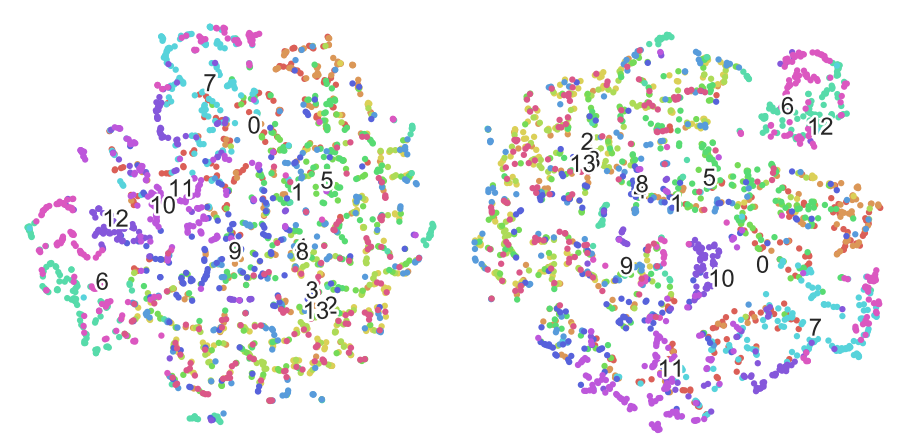
\includegraphics[width=0.8\linewidth]{Images/tsne_results.png}
    \caption{Visualisation des espaces latents via T-Sne: à gauche auto-encodeur classique, à droite auto-encodeur modifié ($\lambda$ = 10)}
    \label{fig:AEmodifTSNE}
\end{figure}

Toujours selon le tableau \ref{fig:AEmodif}, nous avons donc voulu comparer la qualité de représentation pour la classification entre un auto-encodeur à fonction de coût classique ($\lambda = 0$) et à fonction de coût modifiée après finetuning. Nous remarquons ici que la normalisation LDA permet d'obtenir des résultats sensiblement meilleurs aux résultats obtenus par un auto-encodeur général sur les deux jeux de données proposés.

\begin{figure}[H]
    \centering
    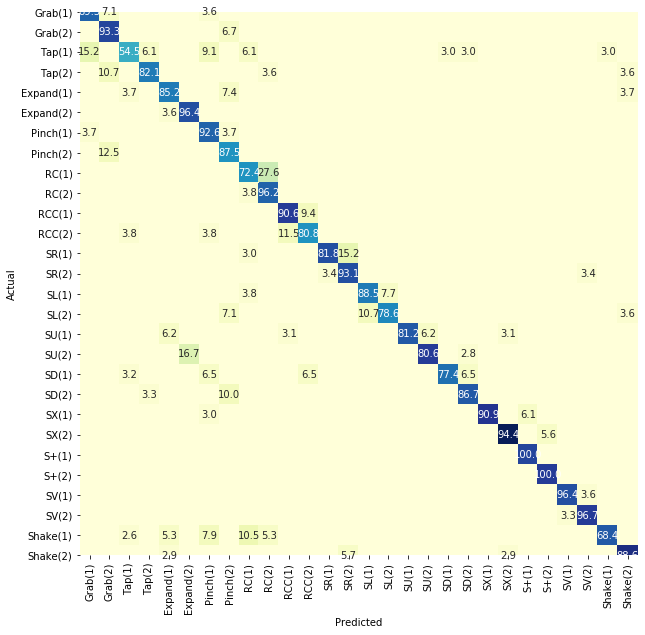
\includegraphics[width=0.8\linewidth]{Images/shrec28.png}
    \caption{Matrice de confusion obtenue sur SHREC 28 avec un auto-encodeur modifié ($\lambda = 5$).}
    \label{fig:rsshrec28}
\end{figure}\textbf{}

Nous avons dans un dernier temps, souhaité comparer l'approche AE-LDA à l'état de l'art pour ces deux jeux de données et ainsi voir si un modèle trivial se focalisant sur la représentation de ses données avec une régularisation non supervisée pouvait concourir avec des approches plus complexes comme les réseaux de neurones à état ou réseau de neurones convolutifs: la figure \ref{fig:tabguillaume} et le tableau \ref{resJHMDB} nous permettent de constater que notre méthode dont les résultats sur SHREC 14 et SHREC 28 sont respectivement 92.5\% et 87.1\% et de 68.3\% sur JHMDB peut jusqu'à une certaine limite concourir avec des approches plus complexes. Il convient cependant de rappeler qu'en se fiant aux résultats de \cite{2019arXiv190709658Y}, notre méthode est jusqu'à 4 fois plus rapide que les méthodes de l'état de l'art (20 000 classifications par secondes).

\begin{figure}[H]
    \centering
    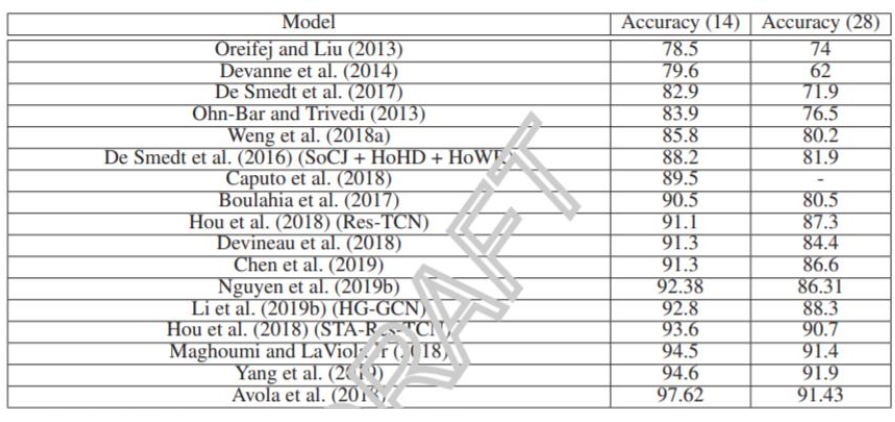
\includegraphics[width=0.8\linewidth]{Images/guillaume_TAB.png}
    \caption{Resultats de l'état de l'art sur SHREC 14/28, image provenant des recherches approfondies sur le jeu de données par Guillaume Devineau. }
    \label{fig:tabguillaume}
\end{figure}\textbf{}

Pour conclure, nous avons montré ici,  qu'il est plus qu’intéressant de se focaliser sur la question de la représentation des données pour la reconnaissance d'action squelettiques. 
\subsection{Perspectives}
Le réseau présenté ci-dessus étant trivial, il est possible d'envisager plusieurs axes d'amélioration:

\begin{itemize}
    \item Essayer plusieurs structures d’auto-encodeur plus travaillées qu'un simple MLP: AE convolutif, AE séquentiel, utiliser des couches d'attention...
    \item Utiliser des analyses factorielles moins spécifiques que l'analyse discriminante linéaire. L'analyse discriminante quadratique par exemple, permettant alors de ne pas émettre de suppositions vis-à-vis des matrices de covariance de chaque classes. 
    \item Cumuler la structuration des keypoints présentée en \ref{dfs} à cette approche pour un auto-encodeur convolutif et évaluer la pertinence de cumuler les deux approches.
    \item L'évaluation de la capacité de génération de l’auto-encodeur n'a pas encore été évaluée.
\end{itemize}

Cependant, nous ne sommes pas complètement convaincus de la capacité de ces deux jeux de données à représenter la totalité des difficultés qui existent pour la prédiction d'intention de piétons. Ainsi, nous avons pour l'instant préféré laisser cette approche en suspens jusqu'à la mise en place d'une pipeline sur des jeux de données de piétons supposément plus complexes.
